\documentclass{article}


\usepackage{amsmath} % math stuff
\usepackage{amssymb} % math stuff
\usepackage{array} % equations and stuff
\usepackage{bm} % bold math
%\usepackage{caption} % suppressed table numbering; incompatible with revtex, and longtable, I think
\usepackage{comment} % comment environment
%\usepackage{enumitem} % customization of enumeration, itemize, and description
\usepackage[T1]{fontenc} % font encoding for special characters, must also use scalable font package
\usepackage[margin=0.8in]{geometry} % paper sizes and margins (but be careful not to mess up pre-defined pages)
\usepackage{graphicx} % for graphics
%\usepackage{helvet} % default font is the helvetica postscript font
\usepackage{lipsum} % lorem ipsum filler text
\usepackage{lmodern} % scalable font?
\usepackage{longtable} % multi-page tables
\usepackage{mathrsfs} % math script font
\usepackage{mhchem} % easier chemical formula
\usepackage{microtype} % allows disabling of ligatures
%\usepackage{newcent} % new century schoolbook font
\usepackage{parskip} % removes paragraph indentation, and adjusts paragraph skip, as well as list items
%\usepackage{setspace} % adjust text spacing and indents
\usepackage{siunitx} % decimal alignment
\usepackage{subfigure} % divided figures
%\usepackage{tabu} % extra table options
\usepackage{textcomp} % symbols
\usepackage{threeparttablex} % better footnotes with longtable
\usepackage{titling} % title placement
%\usepackage{url} % superceded by hyperref
\usepackage{verbatim} % verbatim environment
\usepackage{xcolor} % colors and color boxes
\usepackage{xspace} % commands that don't eat up white space
\usepackage{hyperref} % links and page setup; should always come last

\hypersetup{
	bookmarks=true,
	colorlinks=true,
	citecolor=blue,
	linkcolor=blue,
	urlcolor=blue,
	pdfstartview={XYZ null null 1.0} % default open view is 100%
}

\DisableLigatures[f]{encoding = *, family = * } % disable ff, fi, fl ligatures, without f option, it also disables -- = endash

\begin{document}

\pagestyle{empty} % don't number pages

% custom title
\begin{center}
{\LARGE Riddler Express}

\vspace{0.15in}

{\Large 15 November 2019}
\end{center}


\section*{Riddle:}

\begin{center}
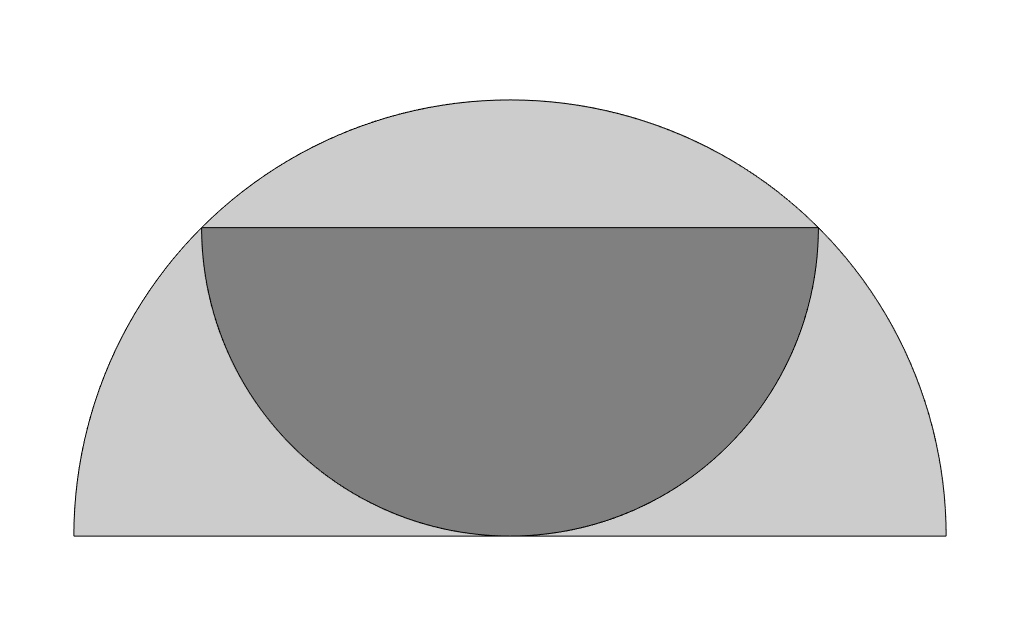
\includegraphics[width=3.5in]{halfcircles.png}
\end{center}

The picture above shows two semicircles.
The lighter region (inside the larger semicircle but outside the smaller one) has an area of 7.
What’s the area of the darker region?


\section*{Solution:}

For this riddle, I am making two seemingly obvious assumptions that make the problem very easy.
First, the small semicircle is tangent at all three points, and second, that the flat edges of the two semicircles are parallel (and exactly horizontal, to wit).
To solve this, I have drawn some lines in the image which make the math clear.

\begin{center}
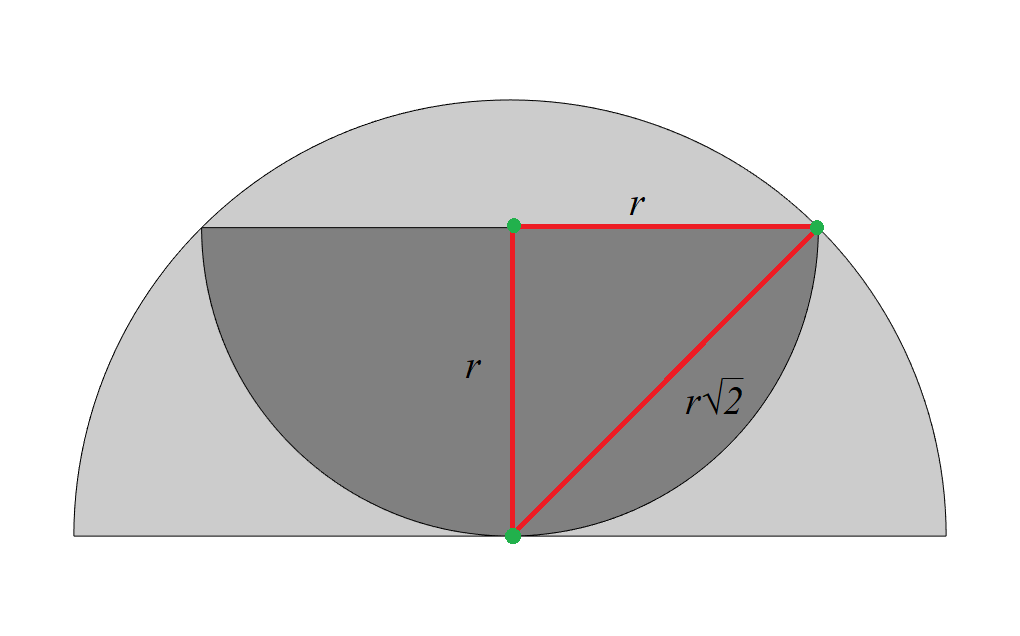
\includegraphics[width=3.5in]{halfcircles_labeled.png}
\end{center}

The small semicircle has radius $r$.
The horizontal and vertical lines are radii, and form a right triangle with hypotenuse $r\sqrt{2}$.
The hypotenuse is also the radius of the larger semicircle, because the centers of the semicircles are vertically aligned.
Therefore, the ratio of the radii is $\sqrt{2}$, and the ratio of the total areas of the semicircles (not just the shaded areas) is 2.
So the total area of the large semicircle is 14, and the remaining lightly shaded area is $14-7$~=
\fcolorbox{red}{white}{\bf 7}\,.


\end{document}